\documentclass[11pt,a4paper]{article}
\usepackage[top=2cm,left=2cm,right=2cm,footskip=0.75in]{geometry}
\usepackage{graphicx}
\usepackage{floatrow}
\usepackage{amsmath,amssymb}
\usepackage{url}
\usepackage[utf8x]{inputenc}
\usepackage{setspace}
\usepackage{multicol}
\usepackage{etoolbox}

\usepackage[slovene]{babel}

\setstretch{1.1}
% \usepackage[document]{ragged2e}
\setcounter{section}{27}  % this is a section 27 of the proposal form

% \setlength{\oddsidemargin}{0.25in}
% \setlength{\textwidth}{6.5in}
% \setlength{\topmargin}{0in}
% \setlength{\textheight}{8.5in}

\newcommand{\myurl}[1]{\footnote{\url{#1}}}

\usepackage{caption}
\captionsetup[figure]{labelfont={bf},name={Fig.},labelsep=period}

\usepackage{fontspec}
\setmainfont{Carlito}

% \usepackage{fontspec}
% \setmainfont[Path=/System/Library/Fonts/,
%     BoldItalicFont=calibriz.ttf,
%     BoldFont      =calibrib.ttf,
%     ItalicFont    =calibrii.ttf]{calibri.ttf}

\renewcommand{\bold}{\textbf}
\graphicspath{ {./images/} }

\begin{document}

\title{\Large Računska orodja za odkrivanje prognostičnih bioloških označevalcev iz podatkov o genskih izrazih: opis raziskovalnega projekta}
\author{}
\date{}
\maketitle
\vspace*{-1cm}

\bold{Predlagamo projekt za oblikovanje in razvoj interaktivne zbirke orodij za pomoč pri iskanju molekularnih prognostičnih bioloških označevalcev (biomarkerjev) iz molekularnih podatkov in podatkov preživetja, pridobljenih v kliničnih poskusih.} V projektu bomo zasnovali računske metode in metode strojnega učenja za iskanje biomarkerjev, jih vključil v interaktivne komponente z grafičnim uporabniškim vmesnikom in zasnovali vizualno programiranje za povezavo teh komponent v cevovode. Razvite metode in zbirka orodij bodo podpirale sodelovanje med podatkovnimi znanstveniki in strokovnjaki s področja razvoja bioloških označevalcev - zdravniki, biomedicinski ali farmacevtski raziskovalci. Z njimi bo možno preiskati podatke o molekularnih odzivih tisočih genov, da bi našli tiste, ki najbolj korelirajo s preživetjem. Predlagano orodje bo dostopalo do obstoječih modelov, ontologij in podatkovnih baz, da bi tako pospešilo interpretacijo in ponudilo polavtomatske razlage rezultatov.

\bold{To je aplikativni projekt, pri katerem se povezujemo z Genialisom, specializiranim podjetjem za podatkovno znanost na področju k posamezniku usmerjene medicine (ang.~{\em precision medicine}).} Genialis je trenutno v postopku registracije pri FDA (Ameriška uprava za hrano in zdravila) prvega modela strojnega učenja, ki za napovedovanje odziva na zdravljenje bolnikov z rakom uporablja podatke o transkripciji. Genialis potrebuje metode, orodja in vizualizacije za pospešitev raziskav, da bo ostalo v vrhu raziskav biomarkerjev in izboljšalo komunikacijo rezultatov s strankami in regulatornimi agencijam. Po drugi strani pa bo projekt predlagatelju omogočil nadaljevanje naših raziskav interaktivnih vizualizacij in strojnega učenja ter uporabo naših novih pristopov k zahtevnemu področju odkrivanja biomarkerjev.

\subsection{Znanstvena izhodišča ter predstavitev problema in ciljev raziskav}

\subsubsection*{Znanstvena izhodišča}

\bold{Projekt bo prispeval nove metode in praktične pristope k raziskovanju podatkov na področju analize preživetja in preučeval, koliko spremenljivk (genov s svojim izražanjem) skupaj vpliva na preživetje.} Analiza preživetja je sklop statističnih metod, katerih namen je določiti pričakovano življenjsko dobo preiskovane populacije. Analiza preživetja proučuje pričakovano trajanje časa do nekega dogodka, recimo ponovne pojavitve raka po kemoterapiji~\cite{pazdur2008endpoints}. Modeli preživetja, vključno z najbolj znanim modelom razmerja tveganja (ang.~{\em hazard ratio}), se nanašajo na čas do dogodka za eno ali več kovariant. V biomedicini so spremenljivke, ki pomembno vplivajo na preživetje, potencialni označevalci, značilnost biološkega sistema, ki ga lahko merimo objektivno in uporabljamo kot kazalnik stanja sistema. Na primer, pri raku lahko označevalci razlikujejo med bolniki, ki se odzivajo na zdravljenje, in tiste, ki se ne.

\bold{Na podlagi markerjev lahko napovemo uspeh zdravljenja in izberemo pravo terapijo za posameznega pacienta. Identifikacija dobrih označevalcev je tako ključnega pomena za razvoj personalizirane medicine.} Ker izboljšanje preživetja neposredno koristi bolniku, je nujno razumeti, kako se udeleženci odzivajo na različne oblike zdravljenja. Zato je treba zdravljenje izbrati glede na bolnikovo stanje in značilnosti, ki so definirane s pomočjo nabora markerjev. Označevalci so lahko klinični, povezani s pacientovimi simptomi, ali biološki, povezani z nekaterimi meritvami na molekularni ravni, kot je koncentracija določenega proteina ali izražanje določenih genov. Označevalci se lahko nanašajo na posamezno meritev ali skupino meritev, po možnosti povezanih s prognostičnim modelom ali omrežjem~\cite{Sonawane2019}.

\bold{Z visokozmogljivim sekvenciranjem lahko merimo stopnjo aktivnosti genov v bioloških vzorcih.
V zadnjih letih se pozornost usmerja s preprostih eno-genskih markerjev na nivoju DNA na kompleksne večgenske označevalce na nivoju izražanja genov.} oličina mRNA v biološkem vzorcu, ki ustreza določenemu genu, je povezana z aktivnostjo gena in se imenuje izražanje genov. Visoko zmogljivo sekvenciranje omogoča določitev izražanje vseh genov v organizmu in tako predstavlja orodje za oceno stanja biološkega sistema. Gen lahko štejemo za biomarker preživetja, če je funkcija preživetja zelo drugačna v subpopulaciji, kjer je gen izražen, v primerjavi s tisto, kjer gen ni izražen (glej sliko~\ref{fig:km-marker}). Ta opredelitev je nejasna, saj zahteva prag za izražanje genov, količinsko opredelitev in naknaden prag razlike med funkcijami preživetja. Poleg tega se skupine genov in ne posamezni geni običajno uporabljajo za zajem različnih biologij v vzorcu, npr. nagnjenosti k nastanku krvnih žil ali pripravljenosti na imunski odziv. Preverjen in učinkovit postopek odkrivanja biomarkerjev, ki temelji na izražanju genov, je lahko neverjetno dragoceno in nujno orodje pri odkrivanju, razvoju in diagnostičnih raziskavah zdravil~\cite{MonforteMcPhail2005}.

\begin{figure}
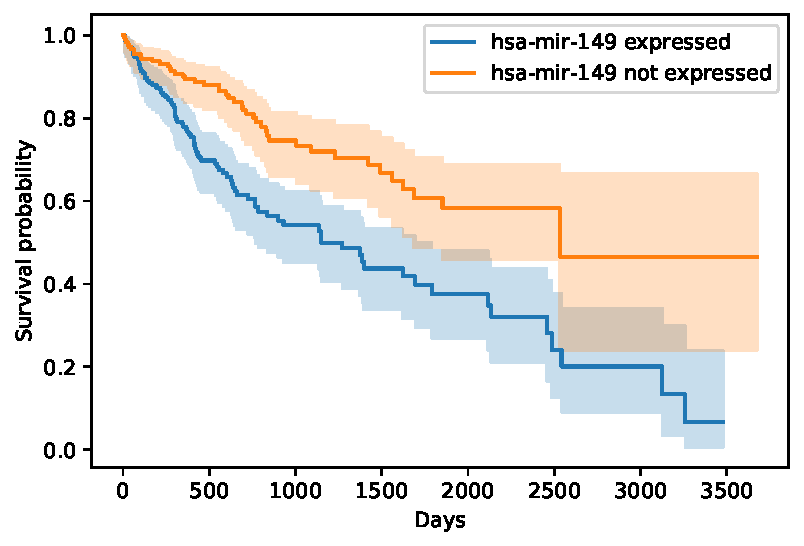
\includegraphics[width=0.48\textwidth]{hsa-mir-149}\hfill
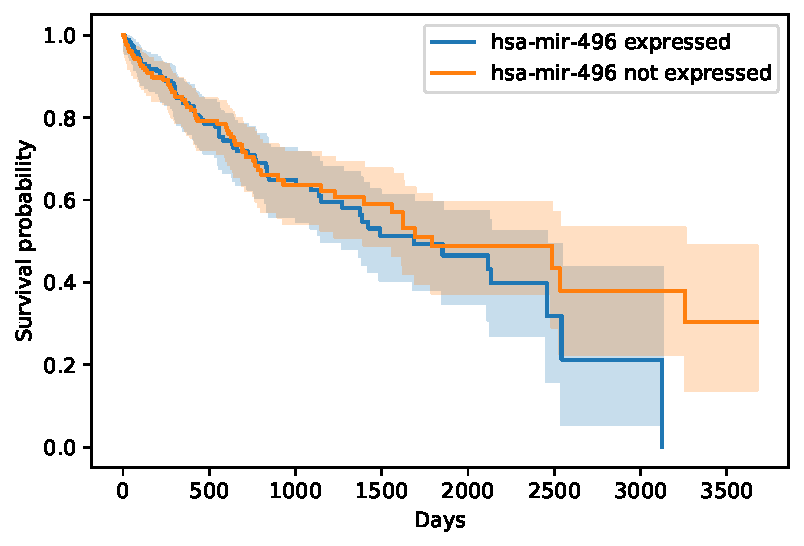
\includegraphics[width=0.48\textwidth]{hsa-mir-496}
\caption{\small\bold{Primer Kaplan-Meierjeve preživetvene krivulje za dve skupini, definirani z izražanjem genov.} Preživetje je bistveno večje pri skupini bolnikov z močno izraženimi
microRNA hsa-mir-149 (leva slika). Razlika pri mikroRNA hsa-mir-496 (desna slika) ni tako očitna. Lahko bi rekli, da je hsa-mir-149 torej boljši biomarker za preživetje. Pri odkrivanju biomarkerjev je ena od nalog razvrščanje genov glede na stopnjo ločevanja skupin z različnim preživetjem.}
\label{fig:km-marker}
\end{figure}

\bold{V idealnem primeru bi torej podatkovno odkritje novih biomarkerjev zahtevalo le podatke o preživetju z ustreznimi profili izražanja genov.} Algoritmi bi nato presejali vse gene in poiskali tiste, ki najbolje opredeljujejo skupine z različnimi funkcijami preživetja. Obstaja pa veliko težav in izzivov v tem postopku povezanih s šumom v podatkih, z majhnim številom preiskovanih vzorcev, z interakcijami med geni in vključevanjem razpoložljivega dodatnega znanja (podatkovnih baz). S tem se ukvarjamo podrobneje v nadaljevanju.

\subsubsection*{Predstavitev problema}

\bold{Predlagani projekt obravnava tri kategorije problemov in izzivov, ki vplivajo na
računske metode za ugotavljanje potencialnih biomarkerjev, pristopov k fuziji podatkov in izvedbe:}
\begin{description}
	\item[Računski izzivi, šum in prekomerno prilagajanje modela učni množici (ang.~{\em overfitting}).] Eksperimentalni podatki za preživetje, povezani z npr. vplivom novega zdravljenja ali zdravila, so pogosto dragi in zato so eksperimentalni vzorci majhni. V tipičnem kliničnem poskusu prve faze je pogosto manj kot 30 bolnikov, v 2. kliničnem poskusu pa je več kot sto bolnikov prej izjema kot pravilo. Podatkovni šum, povezan z načinom zbiranja, obdelavo vzorcev in merjenjem ekspresije genov, je lahko visok. Tako okolje lahko vodi do lažnih odkritij in prekomernega prilagajanja modela učni množici. Težava je še posebej očitna pri iskanju skupin ali mrež genov, ki bi lahko služili kot biomarkerji, saj število kandidatov (različnih skupin genov) raste eksponentno z želeno velikostjo nabora genov za biomarker. Na primer, za $20000$ genov, ki kodirajo beljakovine, obstaja več kot  $1.3$ bilijonov možnih genskih trojk. Tudi če bi nam uspelo vse računsko preučiti, bi to nujno povzročilo prekomerno prilagajanje modela učni množici, zato bi se rezultati dobro opisovali učne podatke, vendar bi se slabo posploševali na nove primere. Poleg šuma in prekomernega prilagajanja modela (ang.~{\em overfitting}) računski izzivi vključujejo še iskanje pragov ekspresije genov (kdaj je gen izražen?) in agregacijske funkcije (kdaj je skupek genov aktiven?).
 	\item[Vključevanje podatkovnih baz.] Geni sodelujejo v molekularnih poteh, funkcionalnih skupinah in odzivih na kemikalije in zdravila. Znanje o tem in druge genske anotacije so shranjene v podatkovnih bazah, kot so GeneOntology\myurl{http://geneontology.org}, KEGG\myurl{https://www.genome.jp/kegg}, CellMarker\myurl{http://biocc.hrbmu.edu.cn/CellMarker} in druge. Preučevanje genskih kompletov kot kandidatov za biomarkerje bi lahko in bi moralo uporabiti te dragocene vire informacij; tako za omejevanje prostora za iskanje biomarkerjev kot za razlago naborov najboljših kandidatnih genov (obogatitev genskega nabora). Takšno združevanje podatkov in baz znanja je že prineslo zanimive rezultate v bioinformatskih raziskavah~\cite{pmid30467459,pmid26465776}, vendar je bilo na področju odkrivanja biomarkerjev preživetja premalo raziskano.
 	\item[Vmesnik za raziskovanje podatkov.] V zadnjih dveh desetletjih so se pojavile različne metode, statistična orodja in orodja za strojno učenje za analizo visoko zmogljivih podatkov iz molekularne biologije. Analizi preživetja pa manjka elegantna zbirka orodij z intuitivnim uporabniškim vmesnikom, ki bi pomagala pri odkrivanju biomarkerjev, podpirala interaktivno analizo raziskovalnih podatkov v realnem času in ponudila enostavno izdelavo analitičnih podatkovnih cevovodov. Na voljo so dobre računalniške knjižnice za analizo preživetja v jezikih R in Python, vendar so to le nepovezani gradniki, ki za uporabo in integracijo zahtevajo napredne programersko znanje. Namesto tega končni uporabniki in znanstveniki s področja potrebujejo orodja za komunikacijo, raziskovanje in modeliranje podatkov ter intuitivna orodja s prilagodljivimi interaktivnimi vmesniki.
\end{description}

\bold{V projektu bomo te tri izzive napadli z razvojem novih tehnik in orodij za interaktivno raziskovanje potencialnih prognostičnih biomarkerjev.} Naš cilj je demokratizirati to področje z razvojem metod in interaktivnega vmesnika za inteligentno analizo podatkov preživetja.

\subsubsection*{Cilji projekta}

\bold{Projekt bo razvil in uporabil nabor računskih orodij za odkrivanje biomarkerjev iz podatkov genskega izražanja in kliničnega preživetja.} Vključili bomo obstoječe pristope k ocenjevanju biomarkerjev na podlagi podatkov o preživetju, modeliranje preživetja in analize obogatitve genskega nabora. Predlagali bomo tudi nove tehnike za analizo preživetja glede na specifične genske interakcije, za izdelavo omrežij markerskih genov in interpretacijo vizualizacij. Razvili bomo metode za hevrističnega iskanje, ki bo uporabljalo objavljene podatkovne baze o genskih funkcijah in presnovnih poteh.

\bold{Projekt bo opolnomočil domenske strokovnjake za uporabo teh orodij v resničnih aplikacijah, v realnem času in brez potrebe po pisanju računalniške kode.} Projekt bo vključeval računske metode v komponente z grafičnim uporabniškim vmesnikom. Izboljšali bomo lastno odprtokodno platformo za rudarjenje podatkov Orange\myurl{http://orangedatamining.com}~\cite{Demsar2013,Curk2005,Godec2019} (slika~\ref{fig:orange-workflow}) z novimi metodami za analizo preživetja. Pokazali bomo, da nastala platforma za vizualno programiranje ne samo bistveno zmanjša zapletenost in čas, porabljen za analizo podatkov, ampak tudi izboljša sodelovanje različnih strokovnjakov z informativnimi vizualizacijami in avtomatsko uporabo domenskega znanja.

\bold{Na koncu bomo predstavili še uporabnost izdelanega orodja.} Uporabili bomo nabor javnih in zasebnih (od sodelujočega podjetja Genialis) podatkov genske ekspresije in ustreznih kliničnih izidov. O uspešnosti projekta se bo presojalo glede na predstavljene primere uporabe in našo zmožnostjo, da nove uporabnike usposobimo za samostojno uporabo razvite tehnologije.

\begin{figure}[htbp]
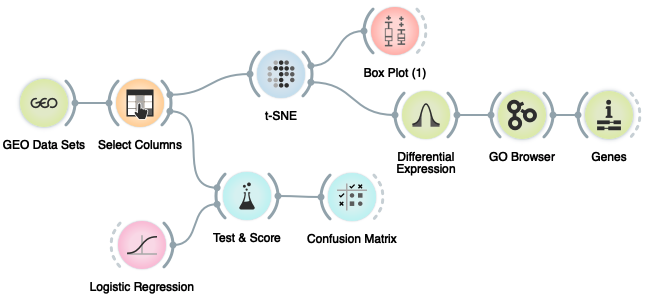
\includegraphics[width=0.7\textwidth]{orange-workflow}
\caption{\small\bold{Tipičen potek dela v programu Orange.} Slika prikazuje primer, ko smo ponovno analizirali gensko izražanje v mononuklearnih celicah periferne krvi. V raziskavi (GDS5363) so avtorji ugotavljali, ali je profiliranje ekspresije genov lahko zaznalo pojav osteoartritisa~\cite{Ramos2014}. Potek dela naloži podatke iz baze Gene Expression Omnibus in definira odvisne spremenljivke (stanje bolezni, izbrane komponente {\em Select Columns}). Zgornja veja postopka preveri strukturo vzorcev tkiva (komponenta {\em t-SNE}), za izbrane vzorce najde različno izražene gene in analizira njihove skupne značilnosti z obogatitvijo izrazov genske ontologije. V spodnji veji preverimo hipotezo preiskovalcev neposredno in ocenimo natančnost napovedi logističnega regresijskega modela s pomočjo navzkrižne validacije (komponenta {\em Test \& Score}). V predlaganem projektu bomo razvili podoben potek dela, vendar s komponentami, ki bodo naložile, obdelale, analizirale in prikazale podatke o preživetju ter predlagale nove biomarkerje.}
\label{fig:orange-workflow}
\end{figure}

\begin{figure}[htbp]
\floatbox[{\capbeside\thisfloatsetup{capbesideposition={right,top},
capbesidewidth=0.37\textwidth}}]{figure}[\FBwidth]
{\caption{\small\bold{Večina grafičnih komponent v programu Orange je interaktivnih.} Tukaj prikazujemo vsebino več komponent iz poteka dela v Sliki~\ref{fig:orange-workflow}. Uporabnik lahko na primer izbere podmnožico podatkovnih točk iz vizualizacije {\em t-SNE} (podatkovne točke z rumenim obrisom zgoraj desno) ali ustrezne podatke v  {\em Box Plot} ali nabor genov, ki so povezani z izbranim izrazom iz modula  {\em GO Browser}. V pripomočku  {\em Differential Expression} lahko izberemo nabor različno izraženih genov v repih porazdelitve. Večina modulov omogoča različne ravni interakcije in medsebojnega povezovanja. Projekt bo nekatere vizualizacijske komponente, vključno s {\em t-SNE}, ponovno uporabil in razvil specializirane, visoko interaktivne module za analizo preživetja in odkrivanje kompleksnih biomarkerjev.}
\label{fig:orange-interactivity}}
{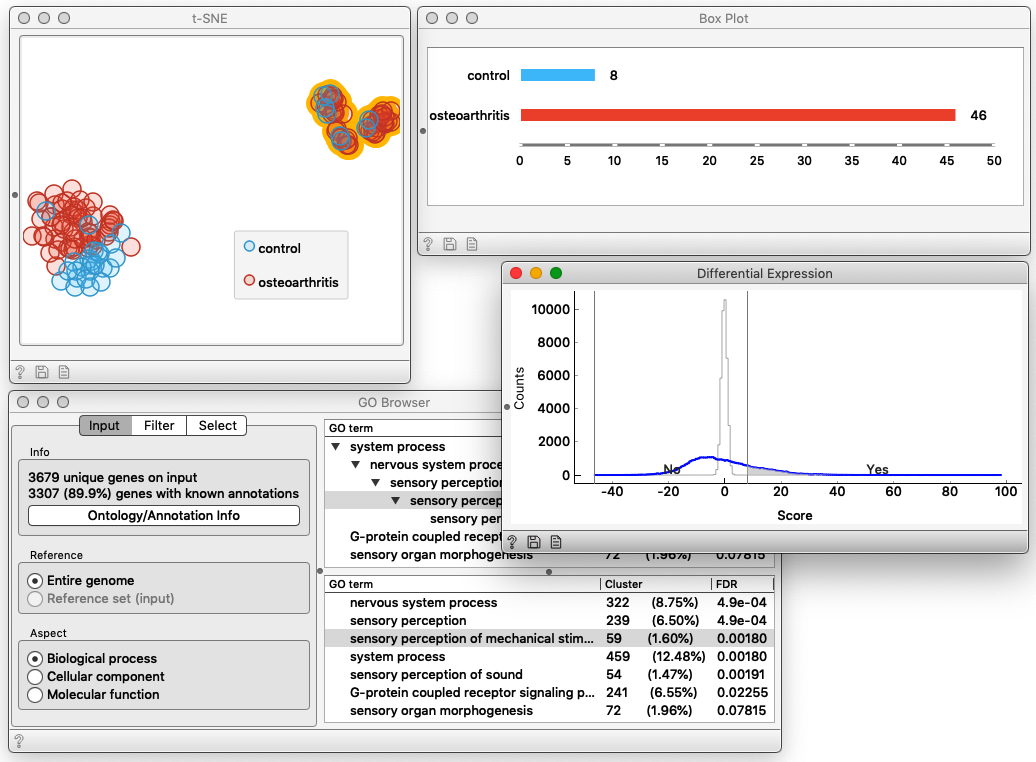
\includegraphics[width=0.6\textwidth]{orange-interactivity}}
\end{figure}

\subsubsection*{Pričakovani rezultati}
Najpomembnejši pričakovani rezultati tega projekta so:
\begin{enumerate}
	\item \bold{XXXXXXXXXXXXX Novi pristopi za odkrivanje biomarkerjev methods and approaches for biomarker discovery}, including computational approaches for survival-based biomarker interaction analysis, visualization approaches to map the space of potential biomarkers, and improved heuristic search for groups of biomarkers through the integration of data and knowledge-bases. XXXXXXXXXXXX
	\item \bold{Knjižnica računalniške kode z metodami za odkrivanje biomarkerjev iz podatkov o preživetju in genskem izražanju.} Knjižnica bo razvita v jeziku Python in bo objavljena v odprtokodni različici na GitHub skupaj z dokumentacijo, testi in primeri uporabe.
	\item \bold{Nabor orodij za odkrivanje biomarkerjev z vmesnikom za vizualno programiranje, interaktivnimi vizualizacijami in razlago rezultatov.} Nabor orodij bomo združili z javnimi podatkovnimi bazami in tako omogočili gradnjo analitičnih cevovodov v realnem času, in interaktivno vizualizacijo podatkov in modelov (glej sliko~\ref{fig:orange-interactivity}), podprto z domenskim znanjem.
	\item \bold{Nabor primerov uporabe, razvit v tesnem sodelovanju z Genialis.} Primeri uporabe bodo prikazali uporabnost naše programske opreme, moč intuitivnega grafičnega vmesnika in zagotoviti učno gradivo za razširjanje rezultatov projekta.
\end{enumerate}

% \subsubsection*{Our Preliminary Results and Studies}

% gene network discovery, gene interactions, intelligent data visualization, embedding, Orange.

\subsection{Pregled literature na področju odkrivanja prognostičnih biomarkerjev}

V literaturi se za primerjavo preživetje med dvema različnima skupinama najpogosteje uporabljata log-rank test in Coxov model sorazmernega tveganja~\cite{singh2011survival}. Ti dve metodi lahko štejemo za izhodišče pri oblikovanju strategij za odkrivanje prognostičnih biomarkerjev. Na kratko, iskanje markerskih genov lahko razdelimo na dva pod-problema: združevanje odzivnih spremenljivk (tu izražanja genov) in iskanje obetavnih skupin genov s prognostično močjo.

V kliničnih študijah so biološki markerji običajno zvezne spremenljivke pridobljene z različnimi meritvami. Vzpostavitev mejne točke, ki predstavlja mejo med visoko in nizko ekspresijo genov ali bolj splošno, ki razlikuje med skupinami z visokim in nizkim tveganjem, je lahko bistvenega pomena za njihovo uporabo pri kliničnih odločitvah~\cite{mazumdar2000categorizing}. Budczies et al.~\cite{budczies2012cutoff} predlagajo več pristopov k izbiri mejnih vrednosti: glede na porazdelitev biološkega markerja z optimizacijo soodvisnosti ciljne spremenljivke, kot je odziv na zdravljenje, ali z iskanjem najmanjše vrednosti p. Slednji je najpogostejši in izbere mejno vrednost glede na optimalno razliko v napovedi izida preživetja med skupinami~\cite{woo2020determination}. Na splošno pa je iskanje optimalne vrednosti težaven problem, ki je odvisen tudi od zasnove študije. Pravilni postopki za določitev mejne vrednosti so zelo pomembni, saj lahko precenimo dejanski učinek biološkega markerja~\cite{Altman1991}.

Witten et al.~\cite{witten2010survival} izpostavljajo problem iskanja napovednih lastnosti v visokodimenzionalnih podatkih. Ko je število spremenljivk veliko večje od števila primerov, običajni statistični pristopi k analizi preživetja niso več zadostni. Obstaja veliko različnih objavljenih pristopov k iskanju marker genov. Nekateri priporočajo dvostopenjsko filtriranje: najprej filtriranje različno izraženih genov (genov, ki se dobro ločijo med izbranimi skupinami) in nato nadaljnje zožitev nabora možnih kandidatov na podlagi statistične pomembnosti pri analizi preživetja~\cite{wang2017identification,liao2018identification,zhang2011discovery,kim2013identification}. Relator et al.~\cite{relator2018identifying} so kritični do takšnih pristopov, ker lahko pustijo številne možne kombinacije genov nepreizkušene. Predlagajo rešitev, ki lahko zazna interakcije potencialnih označevalcev, ki bi jih običajni pristopi izpustili. Pomembna pomanjkljivost njihovega pristopa, kot priznavajo sami, je računska zapletenost. Predlagajo razdelitev podatkov na manjše vzorce, uporabo predlagane rešitve na podvzorcih, in nato kombinacijo rezultatov. Vendar taka rešitev znova lahko izpusti pomembne genske interakcije.

Pri zapletenih boleznih, kot je rak, so učinki izražanja genov na preživetje praviloma nelinearni. Za odkrivanje nelinearnih genskih odnosov so se v zadnjem času pojavili različni pristopi s tehnikami globokega učenja~\cite{hao2019interpretable}. Za napovedovanje preživetja je bilo predlaganih več različnih modelov globokega učenja, vključno s standardnim Coxovovim modelom sorazmernega tveganja (Cox-nnet~\cite{ching2018cox}, SurvivalNet~\cite {yousefi2017predicting}, DeepSurv~\cite{katzman2018deepsurv}). Kljub naprednim tehnikam in povečanju števila potencialnih bioloških markerjev jih je bilo zelo malo klinično uporabljenih~\cite{burke2016predicting}. Če je odkrite označevalce težko razložiti, so ti premalo raziskani ali brez znanih bioloških funkcij, so za kliniko neuporabni. Z modeli globokega učenja je ta izziv toliko večji. Hao et al.~\cite{hao2019interpretable} naredijo korak k iskanju razložljivih skupin genskih markerjev z globokimi nevronskimi mrežami z vključevanjem genomskih in kliničnih podatkov.


Poleg računskih metod se bo predlagani projekt nanašal tudi na obstoječe objavljene prognostične biomarkerje. Na primer, Xiwen et al.~\cite{liao2018identification} in Wang et al.~\cite{33313167} so preučevali korelacije med miRNA in prognozo bolnikov s hepatocelularnim karcinomom (HCC). Oba sta vzpostavila model s podpisi petih miRNA, ki bi lahko služil kot potencialni biomarker pri prognozi bolnikov s HCC. Podobno so Guodong et al.~\cite{31799184} identificirali nov model podpisa s petimi miRNA kot prognostični biomarker pri bolnikih z rakom debelega črevesa in danke. Poleg tega so Martinez-Ledesma et al.~\cite{26202601} raziskali omrežni pristop in identificirali biomarker na osnovi genske ekspresije, ki lahko uspešno napove klinični izid 12 različnih vrst raka. Navedene študije so odličen primer pomena projektov, kot je TCGA. Izčrpni in strukturirani podatki iz baze podatkov TCGA lahko drastično pospešijo razvoj tehnik za odkrivanje (Di et al., \cite{29676997}) in potrjevanje (Chen et al.~\cite{32289666}) obetavnih genskih biomarkerjev.


% \subsubsection*{Computation Methods for Gene Markers Identification in Survival Analysis}
% \subsubsection*{Visual Data Analysis}
% \subsubsection*{Toolboxes}

\subsection{Podroben opis delovnega programa}

\subsubsection{Projektne naloge}

Projekt bo organiziran v okviru naslednjih sklopov nalog:
\begin{description}
	\item[T0] \bold{Vzpostavitev sodelovalnega okolja.} Vso kodo in dokumentacijo bomo odložili na GitHub\myurl{https://github.com/biolab}. Repozitorij bo hranil projektno dokumentacijo in zapisnike sestankov, sledenje spremembam in težavam, knjižnico kode v jeziku Python, teste računalniške kode in primere uporabe. Podatkovne datoteke bodo shranjene na ločen spletni strežnik. Razširitve Orange\myurl{https://orangedatamining.com} bodo razvite kot dodatni paket za namestitev in bodo shranjene v ločenem repozitoriju na GitHubu.
	\item[T1] \bold{Pridobivanje in organizacija podatkov.} Projekt bo uporabil številne različne nabore podatkov, ki prihajajo iz objavljenih študij in zbirk podatkov kot sta NCBI-jev Gene Expression Omnibus\myurl{https://www.ncbi.nlm.nih.gov/geo} in TCGA, The Cancer Genome Atlas database\myurl{https://portal.gdc.cancer.gov}. Poleg tega bomo ustvarili tudi nabor sintetičnih podatkovnih nizov različnih velikosti in zahtevnosti. Zbrani nabori podatkov bodo shranjeni v lastnem repozitoriju, ustvarjenem v nalogi T1.
	\item[T2] \bold{Razvoj orodij podatkovnega rudarjenja in bioinformatike za odkrivanje prognostičnih biomarkerjev.} Še posebej bomo razvijali in izvajali tehnike za:
	\begin{description}
		\item[T2.1] \bold{Razvrstitev in izbiro genov na podlagi funkcije preživetja}, kjer bomo uvedli vse klasične metode s področja, vključno z log rank testom in Coxovim modelom sorazmernega tveganja. Vključili bomo tudi novejše in naprednejše pristope modeliranja, ki temeljijo na naključnih gozdovih (ang.~{\em random forest}) in globokem učenju, ter z njimi rangirali gene in preučevali ubčutljivost različnih pristopov modeliranja.
		\item[T2.2] \bold{Priprava novih spremenljivk}, kjer bomo za agregiranje genske ekspresije uporabili napovedne modele na manjši podskupini genov in s tem povečali robustnost biomarkerja. Uporabili bomo $\ell 1$ regularizacijo v kombinaciji s Coxovim in izpeljanimi modeli, ter pristope z omrežji, pri katerih je biomarker sestavljen iz majhnega števila genov istega regulatornega omrežja ali iste metabolne poti.
		\item[T2.3] \bold{Analiza genskih interakcij}, kjer pričakujemo, da lahko skupina genov deluje nelinearno, da oblikuje močnejši in informativnejši biomarker. Prilagodili bomo pristope k iskanju lastnosti interakcije in pristope za vizualizacijo teh interakcij.
		\item[T2.4] \bold{Omejitve iskanja s podatkovnimi bazami}, kjer bomo omejili iskalni prostor za genske interakcije na skupine genov s skupno funkcijo ali z drugimi skupnimi lastnostmi, kot so opisane v javnih podatkovnih zbirkah, glede na uveljavljene sisteme merjenja ekspresije genov (npr.~nanoString paneli) ali glede na markerjih, znanih iz objavljene znanstvene literature.
 		\item[T2.5] \bold{Globoko in preneseno učenje (ang.~{\em deep learning and transfer learning})}, kjer je naš cilj poiskati genske vložitve (ang.~{\em embedding}) za njihovo profiliranje v prostoru z manj dimenzijami. Avtokoderje (specifične za tkivo in/ali bolezen) bomo trenirali s pomožnimi podatkovnimi seti~\cite{doersch2021tutorial} in jih s prenesenim učenjem~\cite{Godec2019} implementirali na problemu napovedovanja preživetja. Uporabili bomo profile genov v latentnem prostoru za vizualizacijo genskih zemljevidov in hevristično omejitev prostora za iskanje.
 		\item[T2.6] \bold{Zemljevidi interakcije genov}, kjer bi radi predstavili gene -- potencialne biomarkerje -- v genskem  zemljevidu, kjer bližina genov na zemljevidu kaže na povečan skupni učinek na funkcijo preživetja. Ta orodnja bomo gradili na osnovi podobnih metod v analizi podobnega izražanja genov (ang.~{\em coexpression}). Interakcijski zemljevidi bodo zelo vizualno predstavili prostor rešitev pri iskanju določenega biomarkerja.
		\item[T2.7] \bold{Samodejno označevanje točkovnih vizualizacij}, kjer so točke geni, na primer v zemljevidih genskih interakcij. Oblikovali bomo algoritme, ki najdejo soseske z obogateno gensko funkcijo ali presnovnimi potmi, in s tem znanjem avtomatsko anotirali vizualizacije. Te vizualizacije bodo naslednja razvojna stopnja našega predhodnega dela na področju analize izražanja genov v posameznih celicah (glej sliko~\ref{fig:annotation}).
	\end{description}
	\item[T3] \bold{Oblikovanje grafičnih vmesnikov za raziskovalno analizo podatkov o preživetju in odkrivanje biomarkerjev.} V tesnem sodelovanju z Genialisom bomo izvedli temeljito analizo potreb in snovanje končnega produkta, da bi ta zagotovo zasnovan za interaktivno odkrivanje biomarkerjev z integracijo javnih podatkovnih zbirk. Zasnova bo vključevala načrtovanje nabora računskih komponent za obravnavo vseh vidikov analize preživetja in odkrivanjem biomarkerjev. Oblikovali bomo grafični vmesnik, interaktivne vizualizacije in možne cevovode za analizo podatkov. Izvedba bo vsebovala skice grafičnega uporabniškega vmesnika (v Balsamiq Mockups). Poudarek pri zasnovai bo kakovost uporabniške izkušnje, dostop do naprednih računskih tehnik, in zmožnost kombiniranja komponent na način Lego kock pri tvorbi potencialno zelo zapletenih in zmogljivih analitskih postopkov.
 	\item[T4] \bold{Izvedba in integracija.} Razvite računske tehnike bodo implementirane v okviru odprtokodnega okolja za rudarjenje podatkov Orange\myurl{http://orangedatamining.com}. Pri izvedbi bo uporabljena knjižnica metod iz naloge T2 in grafičnih uporabniških načrtov iz T3. Izdelek bo objavljen kot ločen dodatek Orangu in bo sledile uveljavljenim izvedbenim smernicam glede dokumentacije in testiranja vse kode.
 	\item[T5] \bold{Eksperimentalna validacija produkta.} Razvita funkcionalnost bo temeljito preizkušena v sodelovanju z Genialisom, našim projektnim partnerjem. Uporabljeni bodo sintetični in resnični podatki (pripravljeni v okviru naloge 1) ter rezultati primerjani s tistimi iz literature. Validacija bo potrdila veljavnost in pravilnost razvitih postopkov in bo služila za zbiranje študij primerov, ki bodo objavljene na spletnem mestu GitHub, spletni strani Orange ter v načrtovanih publikacijah in patentih.
 	\item[T6] \bold{Razširjanje rezultatov.} Razvite metode bomo objavili pod splošno licenco (GPL). Napisali in spletno objavili bomo ustrezno dokumentacijo z delovnimi primeri, objavili videe s primeri uporabe na Orange YouTube kanalu\myurl{http://youtube.com/orangedatamining} in širili spoznanja s predstavitvami na ustreznih konferencah in v znanstvenih revijah. Ciljali bomo na bioinformatske revije, kot so Bioinformatics, Nature Methods, Artificial Intelligence in Medicine ter konference, vključno z najboljše ocenjenima AIM in ISMB. Načrtujemo tudi prijavo skupnega patenta z Genialisom na področju odkrivanja prognostičnih biomarkerjev.
\end{description}


\begin{figure}
\floatbox[{\capbeside\thisfloatsetup{capbesideposition={right,top},
capbesidewidth=0.37\textwidth}}]{figure}[\FBwidth]
{\caption{\small\bold{Prototip modula v okolju Orange s samodejno anotacijo točkaste vizualizacije.} Na vhodu ta komponenta dobi profil genske ekspresije posameznih celic in njihove vdelave (npr.~koordinate t-SNE) ter seznam markerskih genov za vsak celični tip. V okviru predlaganega projekta bomo uporabil podoben pristop za oblikovanje modula, ki bo pojasnil prostor potencialnih biomarkerjev.}
\label{fig:annotation}}
{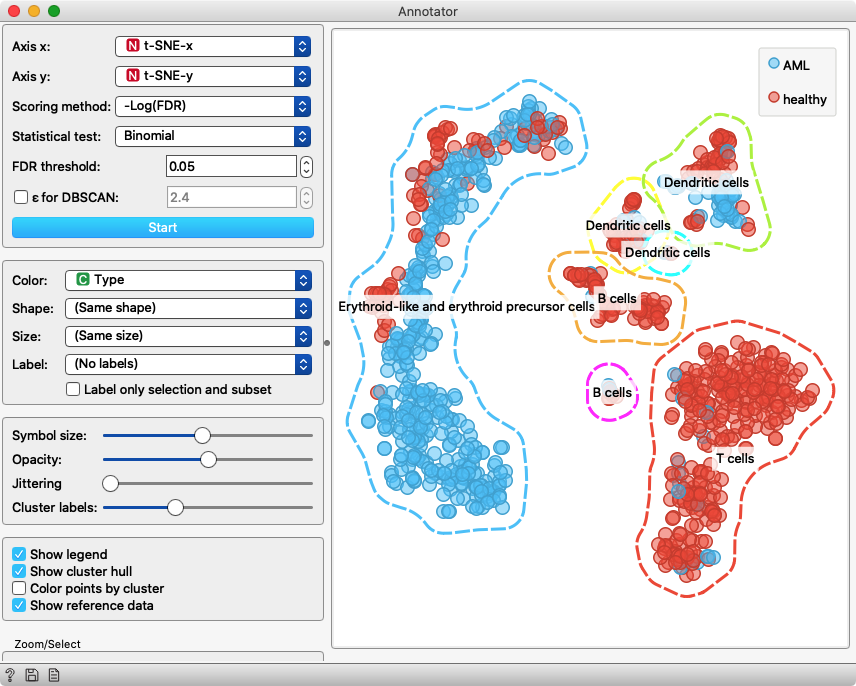
\includegraphics[width=0.6\textwidth]{annotation}}
\end{figure}

\subsubsection{Research Design and Methods}
\begin{description}
	\item[Pregled.] Pregled dela v predlaganem projektu je predstavljen na sliki~\ref{fig:approach}. Slika prikazuje, kako bomo povezali podatke o genskega izražanja in klinične metapodatke z dodatnimi podatkovnimi bazami. Ugotovili bomo
\begin{enumerate}
\item kateri geni so sami po sebi ključni molekularni markerji preživetja,
\item katere kombinacije genov (genski sklopi) so povezane s preživetjem,
\item katere značilnosti markerskih genov nam lahko pomagajo pri interpretaciji rezultatov.
\end{enumerate}
Čeprav bi zgoraj našteta vprašanja lahko individualno in ročno naslovil molekularni biolog, pa jih je v praktičnem smislu mogoče rešiti le s pomočjo računske analize in vključevanjem velikega števila podatkov iz različnih javnih zbirk. Glavni izziv projekta je torej, kako te različne vire združiti in uporabiti sodobne pristope rudarjenja podatkov za predlaganje novih hipotez. V spodnjem opisu najprej navedemo vire podatkov, na katerih bomo uporabili postopek odkrivanja biomarkerjev, nato pa nabor računskih pristopov, ki jih bomo razvili in uporabili, ter komentiramo izvedljivost njihove implementacije znotraj obstoječe platforme za vizualno programiranje Orange.

\begin{figure}
\floatbox[{\capbeside\thisfloatsetup{capbesideposition={right,top},
capbesidewidth=0.37\textwidth}}]{figure}[\FBwidth]
{\caption{\small\bold{Od podatkov do odkritja biomarkerja.} Naš cilj je združiti podatkovni sete s podatki genskem izražanju in kliničnem preživetju z drugimi razpoložljivimi nabori podatkov. Tako bomo pridobili na hitrosti, natančnosti in razlagi rezultatov. Znaten del našega projekta se ukvarja z razvojem grafičnih vmesnikov, ki združujejo vizualizacijo podatkov, biomarkerjev in modelov. Računski in vizualizacijski pristopi bodo postavili rezultate v kontekst celotnega iskalnega prostora (npr. interakcijski zemljevidi) in nam bodo v pomoč pri polavtomatskem procesu odkrivanja novih biomarkerjev. Metode bodo tako podale hipoteze, ki jih bo ocenil domenski strokovnjak, v pomoč pa mu bodo agregirani podatki iz različnih podatkovnih zbirk.}
\label{fig:approach}}
{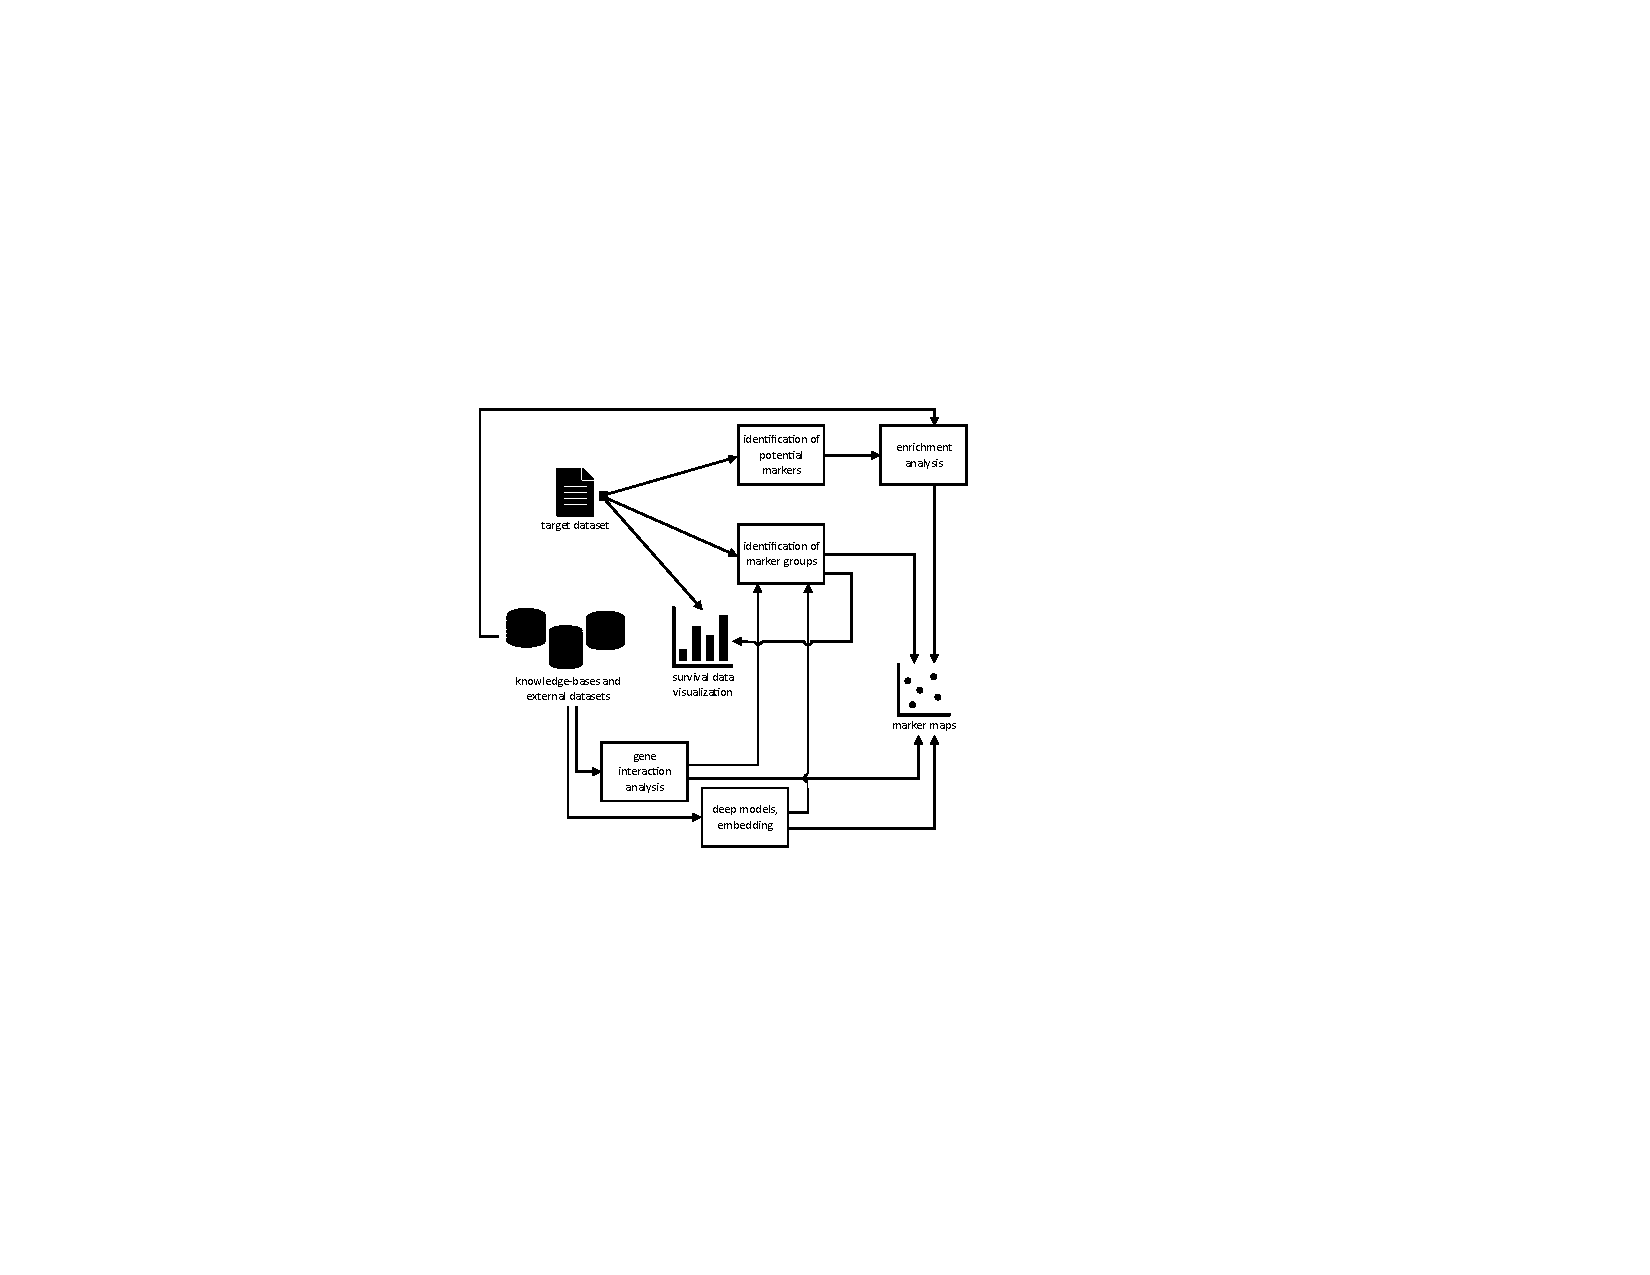
\includegraphics[width=0.6\textwidth]{approach}}
\end{figure}


% \begin{figure}
% 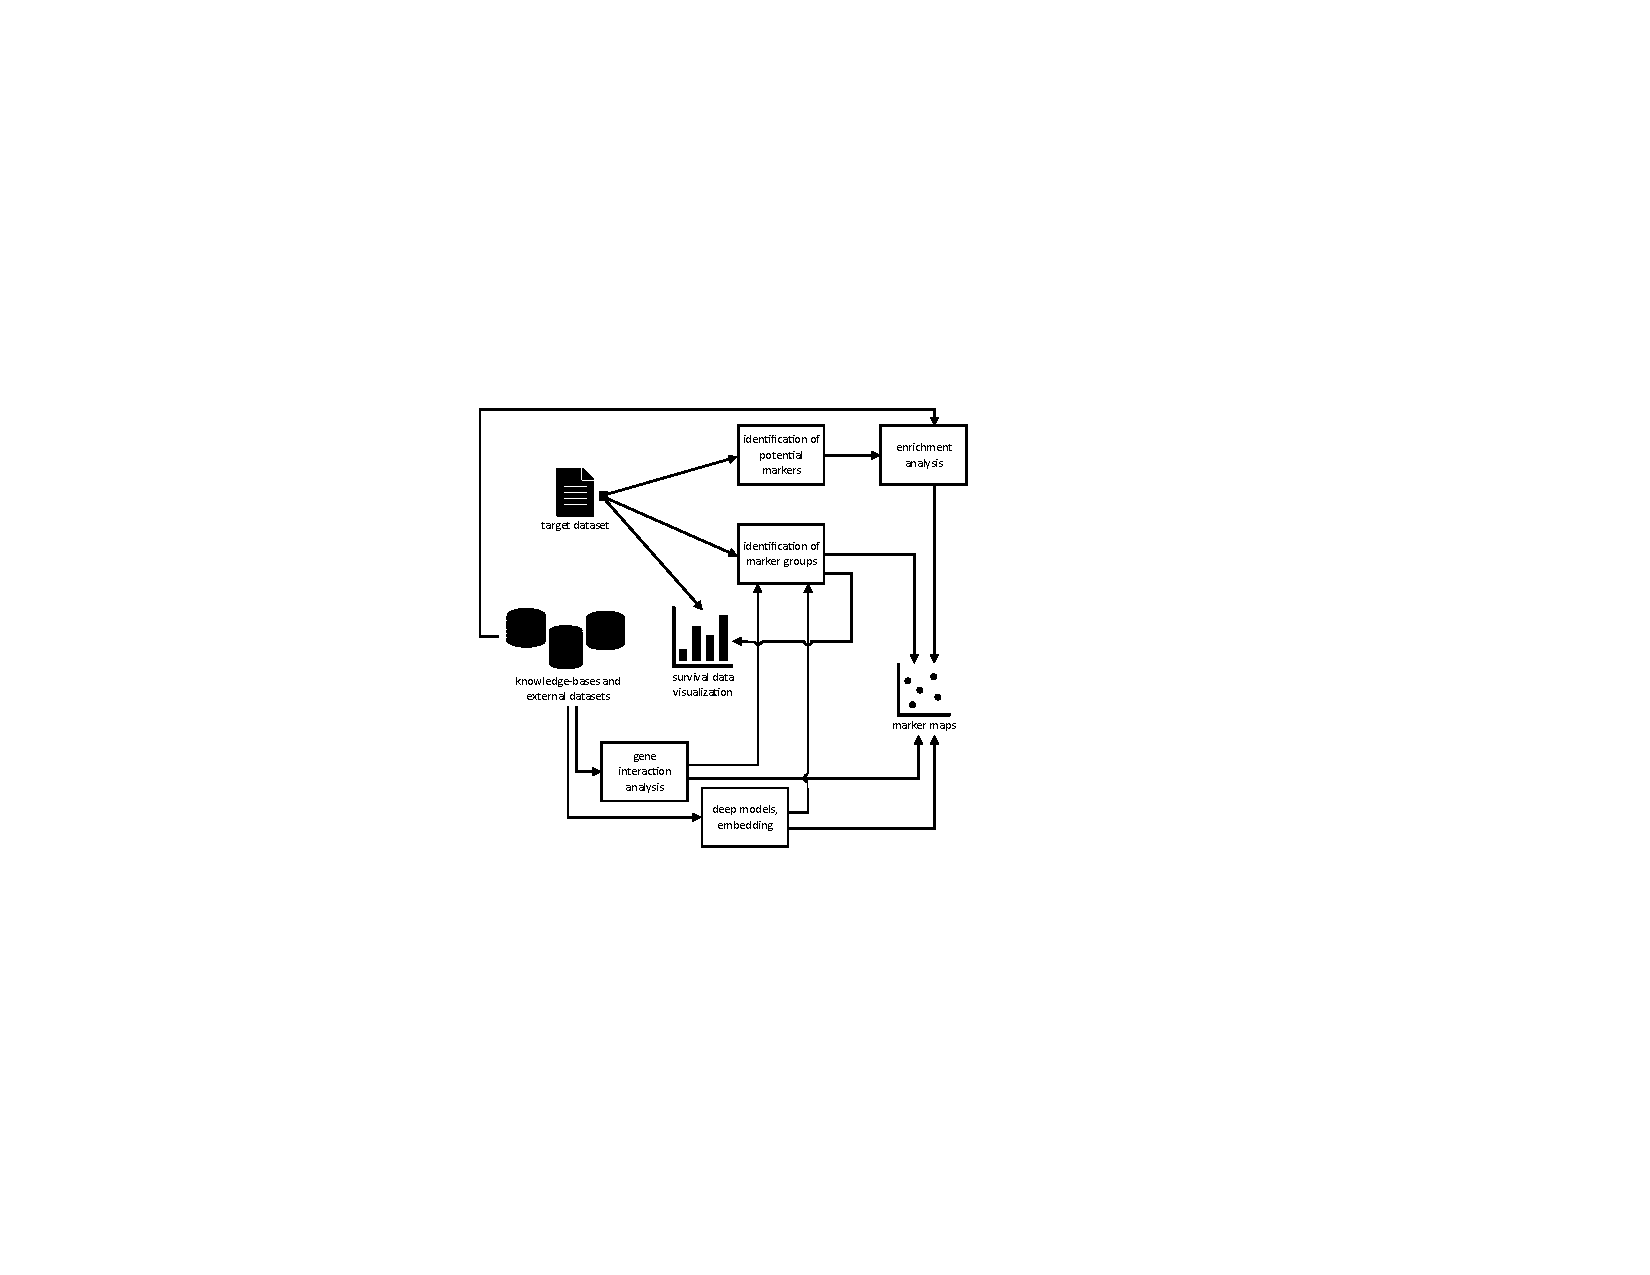
\includegraphics[width=0.48\textwidth]{approach}
% \caption{An example of a Kaplan-Meier plot for two gene expression-dependent conditions associated with patient survival. In panel a), the survival function is substantially higher for a group of patients with highly expressed microRNA hsa-mir-149. The difference is not so evident in the panel b) and microRNA hsa-mir-496. We could say that hsa-mir-149 is hence a better biomarker for survival. In biomarker discovery, one of the tasks is to rank genes and RNA molecules according to the degree of separation between corresponding survival signatures when a gene is expressed and not expressed.}
% \label{fig:approach}
% \end{figure}


	\item[Podatki.] V projektu bodo zbrane, organizirane in uporabljeni štirje viri podatkov o genskih ekspresijah in preživetju:
	\begin{description}
		\item[DS1] Podatki iz baze podatkov The Cancer Genome Atlas\myurl{https://www.cancer.gov/tcga}~\cite{24071849} in Gene Expression Omnibus\myurl{https://www.ncbi.nlm.nih.gov/geo/}~\cite{23193258}.
		\item[DS2] Podatki o analizi preživetja iz kliničnih raziskav iz baze podatkov The Cancer Genome Atlas database.
		\item[DS3] Zasebni podatki o transkripciji in kliničnih preskušanjih, ki jih upravlja Genialis.
		\item[DS4] Simulirani nabori podatkov.
	\end{description}
	Podatki iz DS1 in DS2 so razdrobljeni; nabore podatkov je treba integrirati, tako da so podatki iz kliničnih raziskav poravnani z ustreznimi meta-podatki. Metodološka poročila o razvoju računskih tehnik, vključno s tistimi, ki smo jih navedli v pregledu literature, redko objavijo organizirane podatke, pripravljene za uporabo v prodajnih programskih paketih. Namen projekta je prekiniti s to prakso in sestaviti repozitorij podatkov z usklajenim kliničnim in transkripcijskim podatkovnim nizom, pripravljenem za primerjalno analizo in tehnike odkrivanja biomarkerjev.

	Podjetje Genialis d.o.o. že ima zbirko tovrstnih podatkov, ki izhajajo iz njihovih obstoječih partnerstev z nekaterimi večjimi farmacevtskimi podjetji. Podatki so zasebni, vendar jih bodo v okviru projekta delili z nami za namene razvoja in testiranja.

	Izdelali bomo tudi nabor simuliranih podatkovnih nizov. Podatki bodo služili za testiranje in primerjalno analizo predlaganih metod.

	Projekt bo dodatno uporabil tudi druge vire informacij. Ti vključujejo, vendar niso omejeni na:

	\begin{description}
		\item[DS6] Genske funkcije iz zbirke genskih ontologij konzorcija Gene Ontology (GO).\myurl{https://www.geneontology.org}
		\item[DS7] Presnovne poti iz KEGG, Kjotske enciklopedije genomov in genov.\myurl{https://www.genome.jp/kegg}
		\item[DS8] Podatkovna baza poti NDEx.\myurl{http://www.ndexbio.org/}
		\item[DS9] Različne podatkovne baze markerskih genov, vključno s  CellMarker\myurl{http://biocc.hrbmu.edu.cn/CellMarker}~\cite{cellmarker} in PanglaoDB
		\myurl{https://panglaodb.se}~\cite{30951143}.
	\end{description}

	\item[Računski pristopi, pridobivanje podatkov in bioinformatika] Računski pristopi in razvoj načinov podatkovnega rudarjenja bo vključeval:
	\begin{description}
		\item[Organizacija podatkov (naloga T1).] Projekt bo razvil računalniško platformo z dostopom do skupnih podatkovnih baz s strežniške zbirke, ki bodo hranile podatke o genskem izražanju in preživetju. Za to arhitekturo bomo uporabili običajne prakse programskega inženirstva (podatkovni strežnik z varnim dostopom HTTP, poizvedbe, ki temeljijo na HTTP, komponente na odjemalcih podatkov). Lokalno bomo shranili druge vire informacij, kot so genske ontologije in poti, da bodo te informacije hitro na voljo. Za njihovo ponovno uporabo bomo uporabili obstoječo arhitekturo Orange~\cite{Demsar2013,Curk2005,Godec2019}. Na splošno je cilj skriti kompleksnost dostopanja do podatkov pred uporabnikom. Uporabniki bi morali imeti možnost dostopanja do teh funkcij z enim samim klikom in se osredotočiti na analizo in interpretacijo podatkov.
		\item[Razvrstitev genov (T2.1).] Za primerjavo dveh ali več krivulj preživetja bomo uporabili standardni log-rank test in tako ocenili informacijsko vrednost izbranih genovin prag njihovih ekspresije. Napredni modeli bodo vključevali naključne gozdove~\cite{22088987} in globoko učenje~\cite{katzman2018deepsurv,ching2018cox}. Posredne vrednosti prispevkov posameznih genov bomo določevali z metodami teorije iger, npr. SHAP\myurl{https://github.com/slundberg/shap}~\cite{32607472}.
		\item[Analiza obogatitve genskega sklopa (del T2.1).] Za interpretacijo rezultatov razvrstitve biomarkerjev bomo uporabili analizo obogatitve genskega nabora~\cite{1239896} in pregledali skupne točke najbolje uvrščenih genov glede na funkcije in poti.
		\item[Konstrukcija novih spremenljivk in identifikacija naborov genov (naloga T2.2).] Uporabili bomo neposreden in posreden izbor. Kakovost nabora gena bo ocenjena s pomočjo kvalitete napovedi preživetja. Kot alternativni pristop bomo uporabili izbiro lastnosti z modelom, kot je $\ell 1$ regularizacija Coxovih modelov in modelov omrežja.
		\item[Analiza interakcije genov (T2.3)] bo preučila možne kombinacije genov na njihov skupni učinek na funkcijo preživetja. Nameravamo uporabiti modelno vrednotenje genskih parov (T2.1) in predstaviti rezultate v interakcijskih zemljevidih (T2.6) in omrežjih.
		\item[Odkritje biomarkerja s pomočjo drugih podatkov (T2.4)] bo omejilo iskanje uporabnih kombinacij v nalogi T2.2 na gene s skupno biološko funkcijo, po možnosti na tiste, ki so že povezani s preučevano patologijo v literaturi. Uspeh tega pristopa se bo meril s povečanjem hitrosti algoritma in zmanjšanjem prostora za iskanje, ki ga je treba upoštevati, s tem da bomo zahtevali podobno kakovost rezultatov kot tistih iz izčrpnega iskanja.
		\item[Globoko učenje (T2.5)] bo za vdelavo uporabljalo avtoenkoderje, ki bodo predstavljali kandidate za biomarkerje z vektorji v latentnem prostoru, kjer lahko enostavno pregledamo njihovo povezanost in strukturo prostora biomarkerjev. Iz zbirke transkripcijskih podatkov in naborov kliničnih podatkov (naloga T1) bomo izdelali avtokoderje in nato uporabili prenosno učenje~\cite{Godec2019} za prilagoditev modela določenemu ciljnemu naboru podatkov. Take predstavitve potencialnih markerjev bodo osnova za oblikovanje interpretativnih vizualizacij (npr. naloga T2.6).
		\item[Zemljevidi o interakcijah genov (T2.6)] bodo podajali informacije iz nalog T2.3 in T2.7 z namenom vizualne interpretacije rezultatov. Za upodabljanje genskih zemljevidov bomo uporabili lastno različico t-SNE~\cite{vanDerMaaten2008}, imenovano openTSNE\myurl{https://github.com/pavlin-policar/openTSNE}~\cite{policar2019}, ki lahko ohrani globalno strukturo.
		\item[Razlaga točkovnih vizualizacij] bo opremila genske zemljevide (naloga T2.6) in druge vizualizacije s funkcijskimi oznakami in oznakami presnovnih poti. Ta pristop bomo uporabili za pomoč pri interpretaciji iskalnega prostora. Da bi razvili to tehniko, bomo razširili naš pristop, ki smo ga prej razvili za analizo izražanja genov v posameznih celicah (glej sliko~\ref{fig:annotation}).
	\end{description}

	\item[Uporaba programske opreme.] V zadnjih dveh desetletjih smo razvijali obsežno analizo podatkov z imenom Orange\myurl{https://orangedatamining.com}~\cite{Demsar2013,Curk2005,Godec2019}. Orange uporablja tisoče uporabnikov po vsem svetu in je izbrano orodje pri izobraževanju podatkovnih znanosti na stotinah univerz\myurl{https://orangedatamining.com/blog/2021/2021-01-11-orange-in-classroom/}. Orange ima skriptni del in vizualno programsko okolje. Vizualno programiranje ponuja intuitivno sredstvo za kombiniranje orodij analiz in vizualizacij v zmogljive aplikacije. Orange vsebuje nabor vizualnih komponent za funkcijsko genomiko (slika~\ref{fig:orange-interactivity}), ki uporabnikom, ki niso programerji, omogoča analizo transkripcijskih podatkov in prilagoditev njihove analize s kombiniranjem običajnih orodij za analizo podatkov, ki ustrezajo njihovim potrebam~\cite{Godec2019}. Orodje Orange bomo uporabili za razvoj metod, ki jih predlagamo v projektu, in jih bomo delili z znanstveno skupnostjo znotraj odprtokodnega modela.

	V okviru projekta bomo razvili nabor komponent, ki bodo specifične za naš problem, hkrati pa dovolj splošne za druge naloge iz analize preživetja. Razviti želimo komponente za modeliranje preživetja, oceno natančnosti, razvrstitev biomarkerjev, identifikacijo skupin markerjev, vgradnjo (ang.~{\em embedding}) genov in izdelavo zemljevidov genskih interakcij na osnovi preživetja. Orange že vsebuje nekatere gradnike, ki so ključnega pomena za predlagani projekt. Te vključujejo dostop do knjižnic genskih pripisov, obogatitve genskega nabora, brskalnika GO in orodij za vizualizacijo, vključno z vizualizacijama t-SNE in krivulj Kaplan-Meier.

	\item[Eksperimentalna potrditev.] Podatke DS1 do DS4 bomo uporabili za eksperimentalno potrditev računskih tehnik in vizualnih vmesnikov. Ocenjevali bomo tri vidike:
	\begin{itemize}
		\item \bold{napovedna uspešnost}, kjer bomo primerjali napovedi biomarkerjev z znanimi biomarkerji in primerjali rezultate naših tehnik odkrivanja markerjev z objavljenimi;
		\item \bold{razumljivost}, ki jo bodo ocenili domenski eksperti, ki sodelujejo z Genialisom.
Ocena razumljivosti bo kvantitativna glede na to, kako dobro lahko identificirane biomarkerje povezujemo z znanimi funkcionalnimi genskimi potmi, in subjektivna v smislu potrditve napovedanih genskih poti s strani domenskih ekspertov;
		\item \bold{uporabnost}, kjer bomo z domenskimi eksperti na praktičnih delavnicah ocenili, ali lahko po triurnem treningu orodje uporabljajo samostojno.
	\end{itemize}
\end{description}

\subsection{Razpoložljiva raziskovalna oprema nad 5.000 €}

Genialis bo prispeval spletno orodje Genialis Expressions (glej sliki~\ref{fig:genialis-expressions-frontend} in~\ref{fig:genialis-expressions-software-components}) za agregacijo, pregledovanje in analizo podatkov genskih zaporedij ter kliničnih in eksperimentalnih podatkov. Orodje Genialis Expressions je nameščeno na spletno platformo Amazon AWS Kubernetes in je v lasti podjetja Genialis.

\begin{figure}[htbp]
\floatbox[{\capbeside\thisfloatsetup{capbesideposition={right,top},
capbesidewidth=0.24\textwidth}}]{figure}[\FBwidth]
{\caption{\small\bold{Genialis Expressions} je spletno stičišče biomedicinskih podatkov, ki zagotavlja principe dostopnosti, interoperabilnosti in ponovne uporabe podatkov (angl. FAIR principles -- Findable, Accessible, Interoperable and Re-usable). Podpira avtomatsko primarno analizo podatkov geniskih sekvenc, hrani informacijo o izvoru podatkov in omogoča ponovljivost računskih analiz. Genialis Expressions omogoča sodelovanje uporabnikov, ki lahko podatke izmenjujejo, in podpira integracijo s poljubnimi programi kot je npr.~Orange.}
\label{fig:genialis-expressions-frontend}}
{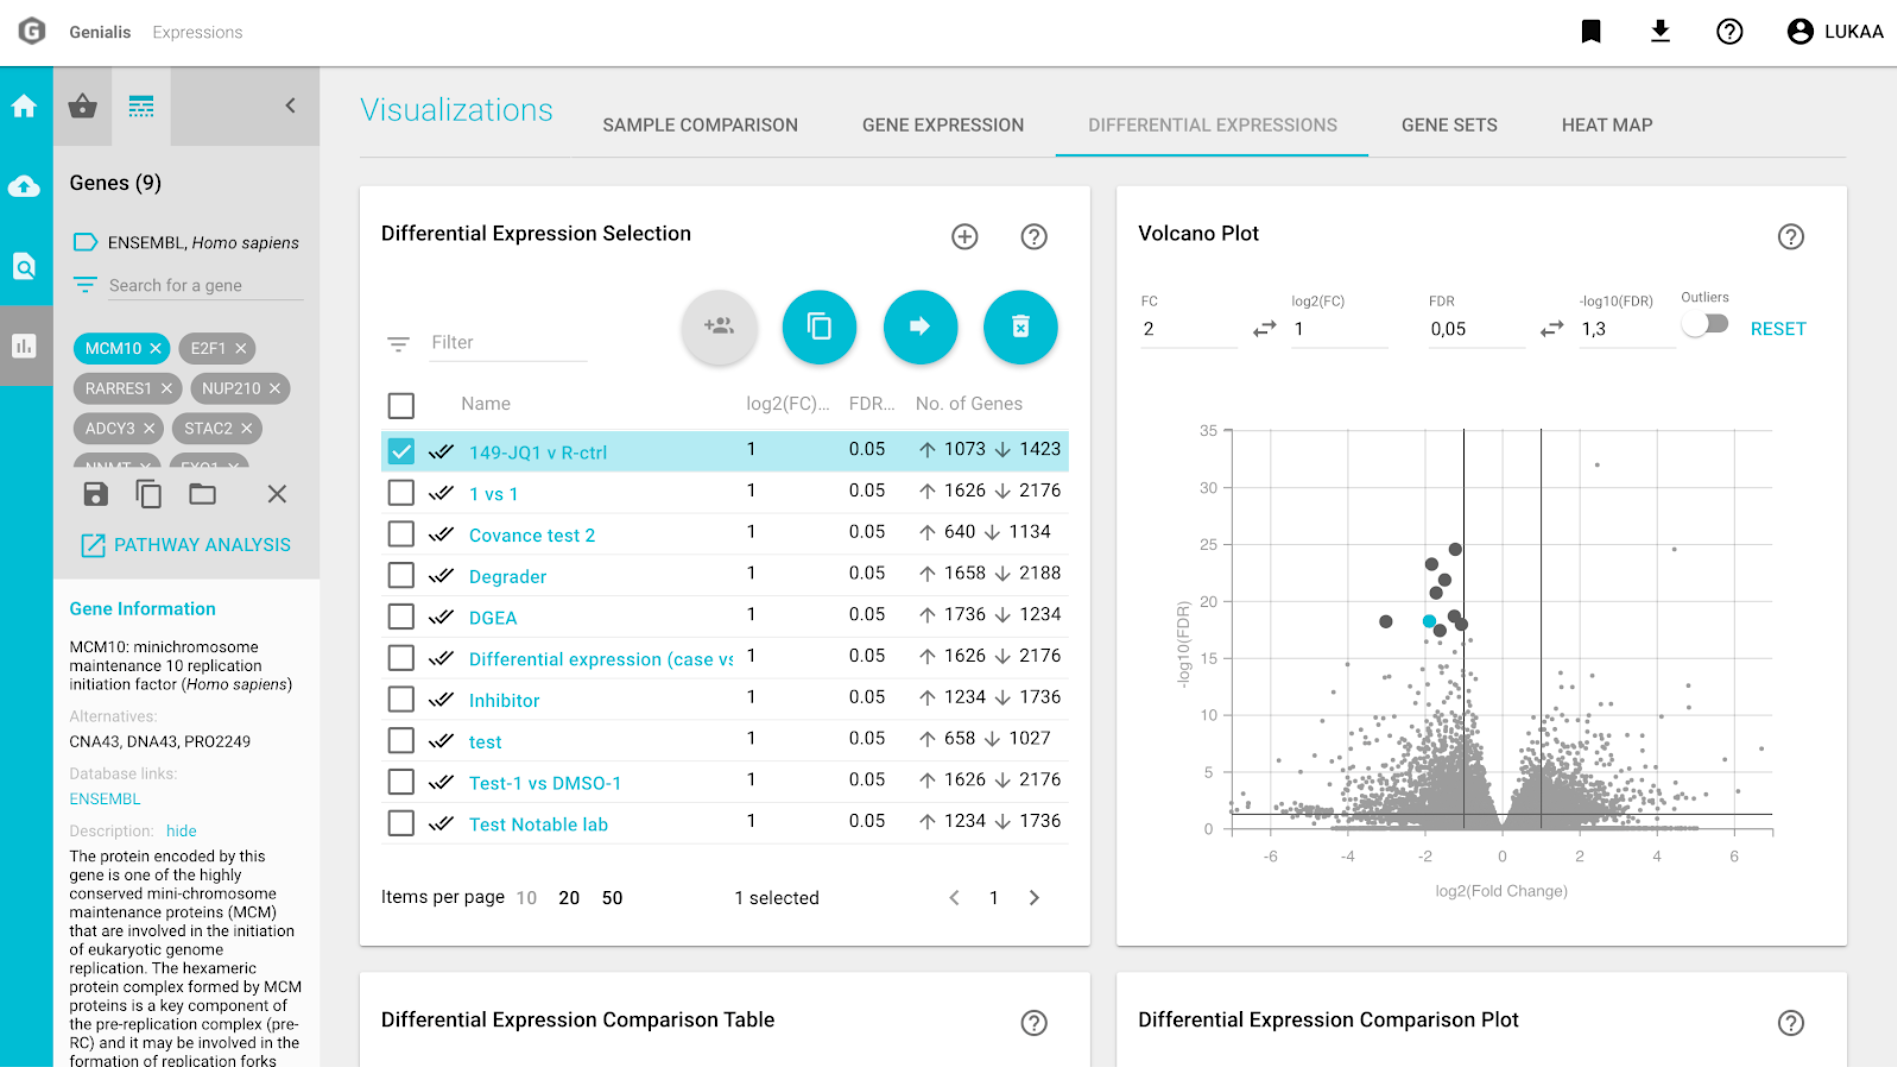
\includegraphics[width=0.73\textwidth]{genialis-expressions-frontend}}
\end{figure}

\begin{figure}[htbp]
\floatbox[{\capbeside\thisfloatsetup{capbesideposition={right,top},
capbesidewidth=0.2\textwidth}}]{figure}[\FBwidth]
{\caption{\small\bold{Genialis Expressions ima modularno arhitekturo programske opreme.} Prednja plast (angl. frontend) komunicira z zaledjem (angl. backend) preko vmesnika RESTful API. Na voljo so knjižnice za razvoj povezane programske opreme v programskih jezikih TypeScript in Python, na primer za integracijo s programom Orange kot je prikazano s sivo barvo v zgornjem desnem kotu. Tudi komponente za podatkovno analizo imajo modularno zasnovo (glej rjava polja na sliki desno). Analize tečejo vzporedno v gruči računalnikov Kubernetes, vsaka v svojem izoliranem okolju v vsebnikih Docker.}
\label{fig:genialis-expressions-software-components}}
{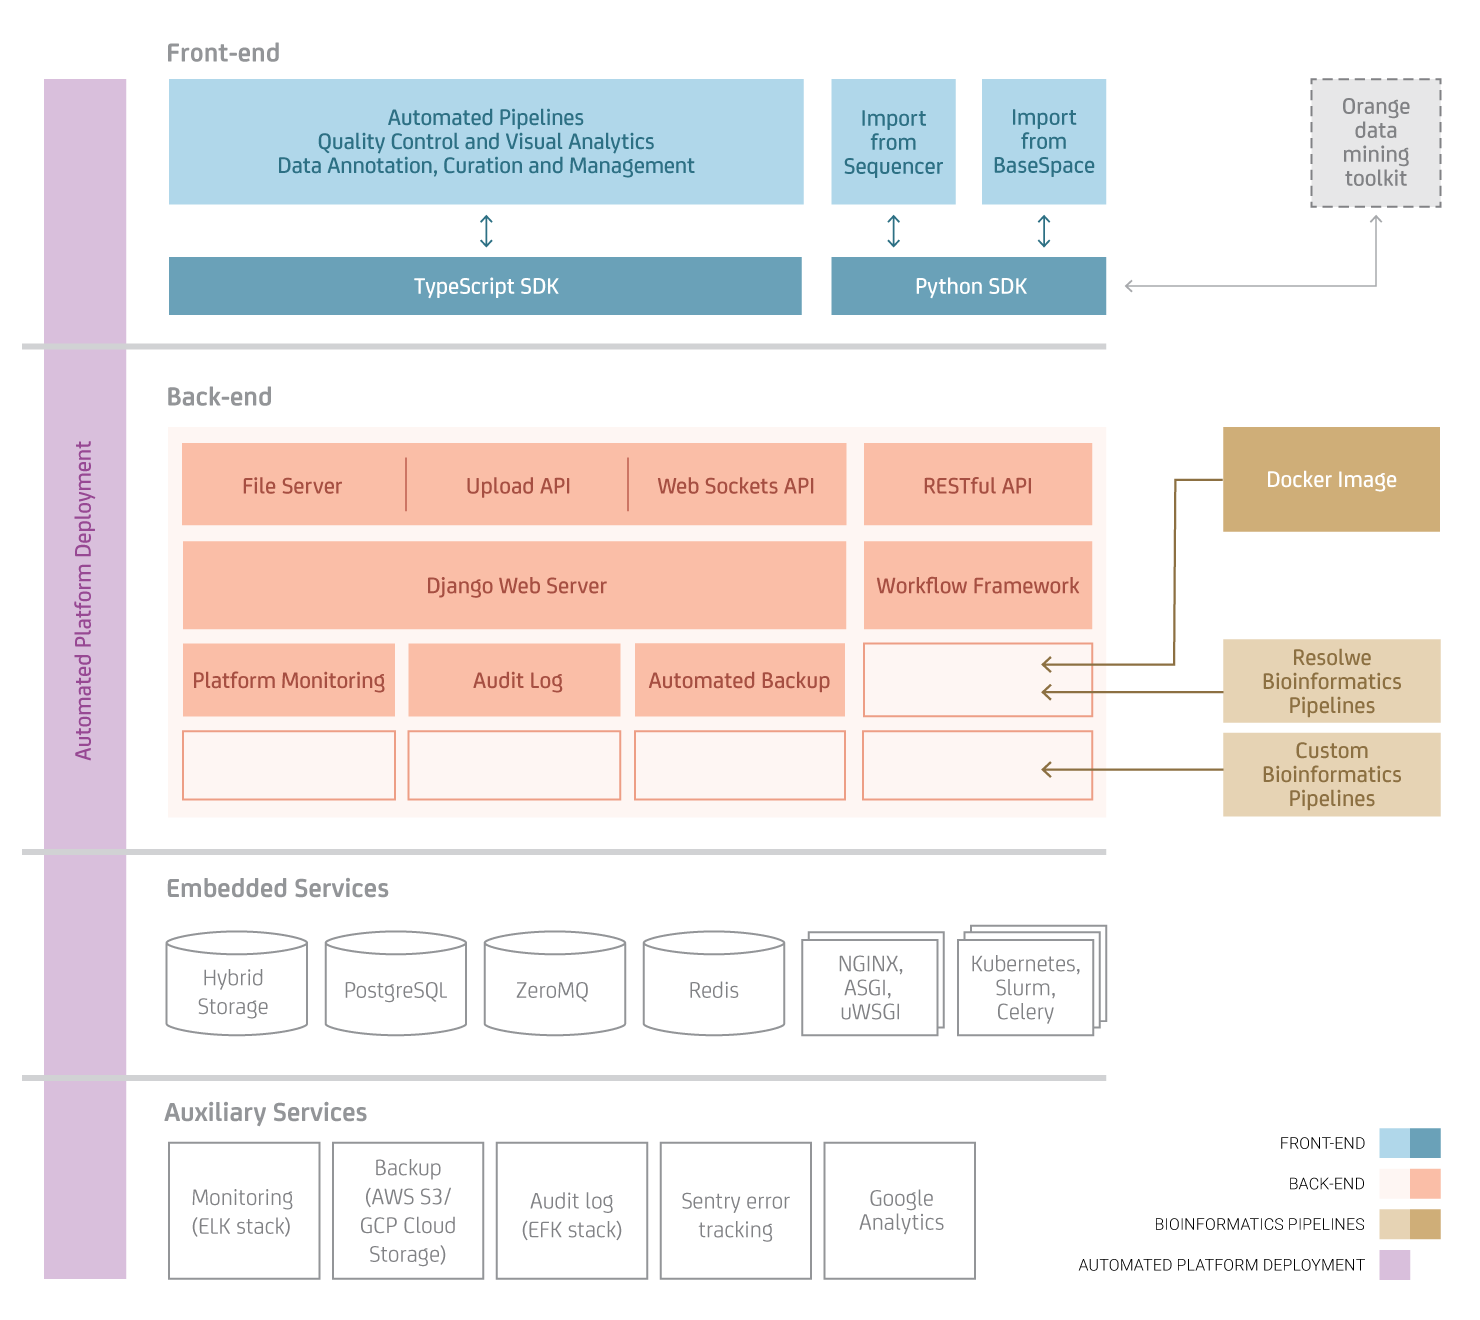
\includegraphics[width=0.8\textwidth]{genialis-expressions-software-components}}
\end{figure}

Projekt bo uporabljal računalniško infrastrukturo Laboratorija za bioinformatiko Univerze v Ljubljani, ki vključuje računalniško gručo z računskimi procesorji CPU (približno 500 procesorjev), pomnilnik NFS (približno 500 TB) in računalniško gručo z grafičnimi procesorji GPU (približno 20 grafičnih procesorjev) v skupni vrednosti približno 200.000 EUR. Za predlagani projekt ne bomo potrebovali posebne računske opreme poleg obstoječe.

\subsection{Vodenje projekta}

Projekt bo združil dve komplementarni skupini raziskovalcev iz univerze in gospodarstva. Laboratorij za bioinformatiko Univerze v Ljubljani prinaša široka strokovna znanja na področjih rudarjenja podatkov, strojnega učenja, bioinformatike in računskega fenotipiziranja. Projekt bo sofinanciralo podjetje Genialis, ki raziskuje in trži nove pristope zdravljenja bolezni, na področjih klinične in translacijske medicine. Genialis sodeluje s farmacevtskimi podjetji pri identifikaciji tarč, iskanju in razvoju biomarkerjev in pozicioniranju novih zdravil. Skupaj so razvili nove pristope za odkrivanje zdravil in zdravljenj, ki bistveno izboljšajo kakovost življenja ljudi z zapletenimi boleznimi.

Projekt bo vodila UL (vodja projekta). Vodenje projekta bo organizirano na rednih sejah upravnega odbora s po enim imenovanim predstavnikom iz vsake institucije in z rednimi sestanki članov projekta. Platforma za sodelovanje bo temeljila na GitHub in bo na razpolago že v zgodnejši fazi projekta.

Projekt bomo zaključili v treh letih. Slika~\ref{fig:gantt} prikazuje podrobno časovnico projekta.

\begin{figure}
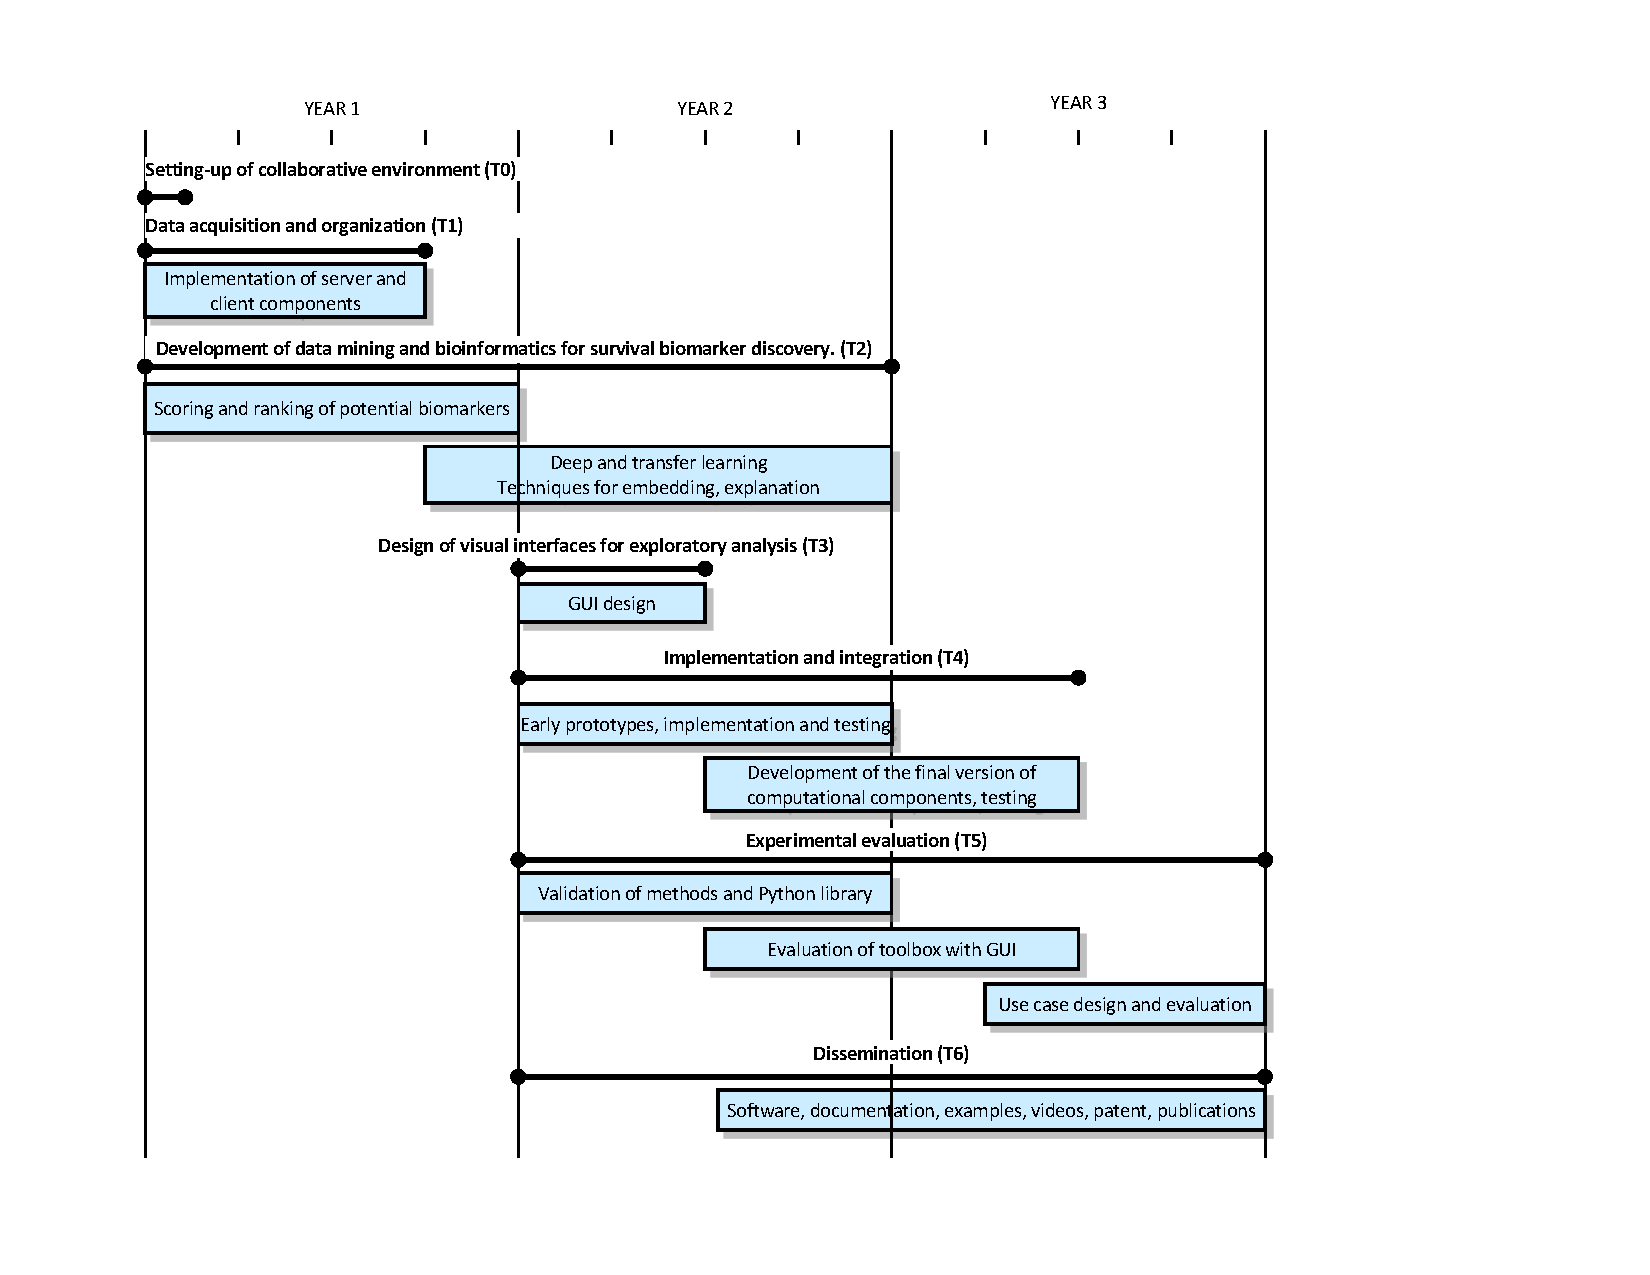
\includegraphics[width=0.90\textwidth]{gantt}
\caption{\small\bold{Časovnica projekta}. Začeli bomo z urejanjem podatkov. Nato bomo razvili Python knjižnico za odkrivanje genskih markerjev pri analizi preživetja. Nadaljevali bomo z načrtovanjem in izvedbo grafičnega uporabniškega vmesnika za nove komponente knjižnice podatkovnega rudarjenja Orange. V sodelovanju z Genialisom bomo testirali komponente na realnih problemih. Posebno pozornost bomo namenili  diseminaciji rezultatov, vključno z objavo odprtokodne programske opreme, dokumentacije, primerov uporabe, video materialov, znanstvenih objav in vložitvijo patenta.}
\label{fig:gantt}
\end{figure}

% \clearpage
\subsection*{Reference}

\patchcmd{\thebibliography}{\section*{\refname}}{}{}{}

\begin{multicols}{2}
\footnotesize
\setlength{\parskip}{0em}
\renewcommand{\baselinestretch}{1.0}
\bibliographystyle{abbrv345}
\bibliography{main}
\end{multicols}

\end{document}
